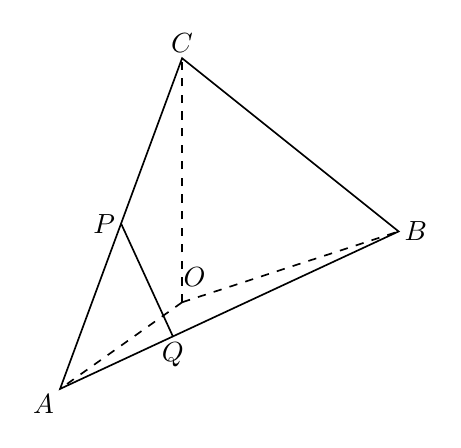
\begin{tikzpicture}[x=1cm,y=1cm,font=\normalsize,
  geometry edge/.style={solid,line width=.6pt},
  geometry label/.style={font=\normalsize,inner sep=2pt}]
\coordinate (A) at (0,0);
\coordinate (O) at (1.5500000000,1.1000000000);
\coordinate (C) at (1.55,4.2);
\coordinate (B) at (4.3,2.0);
\coordinate (P) at (0.775,2.1);
\coordinate (Q) at (1.4333333333,0.6666666667);
\draw[geometry edge] (A)--(C)--(B)--cycle;
\draw[geometry edge] (P)--(Q);
\draw[geometry edge,dashed] (O)--(C);
\draw[geometry edge,dashed] (O)--(B);
\draw[geometry edge,dashed] (O)--(A);
\node[geometry label,below left] at (A) {$A$};
\node[geometry label,above] at (C) {$C$};
\node[geometry label,right] at (B) {$B$};
\node[right=2pt,xshift=-5pt,yshift=9pt] at (O) {$O$};
\node[geometry label,left] at (P) {$P$};
\node[geometry label,below] at (Q) {$Q$};
\end{tikzpicture}
